% Fundamental domain defined by Fourier mode in KS equation.
% use package tikz
% By Xiong
%
% use the following command to generate the pdf
% pdflatex --jobname=ksFund-f1 ksFund.tex

\documentclass{article}
\usepackage{graphicx}
\usepackage{tikz}
\usetikzlibrary{calc}
\usetikzlibrary{arrows}
\usetikzlibrary{decorations.markings}
\usetikzlibrary{decorations.pathreplacing}

\pgfrealjobname{ksFund}


\begin{document}

\beginpgfgraphicnamed{ksFund-f1}
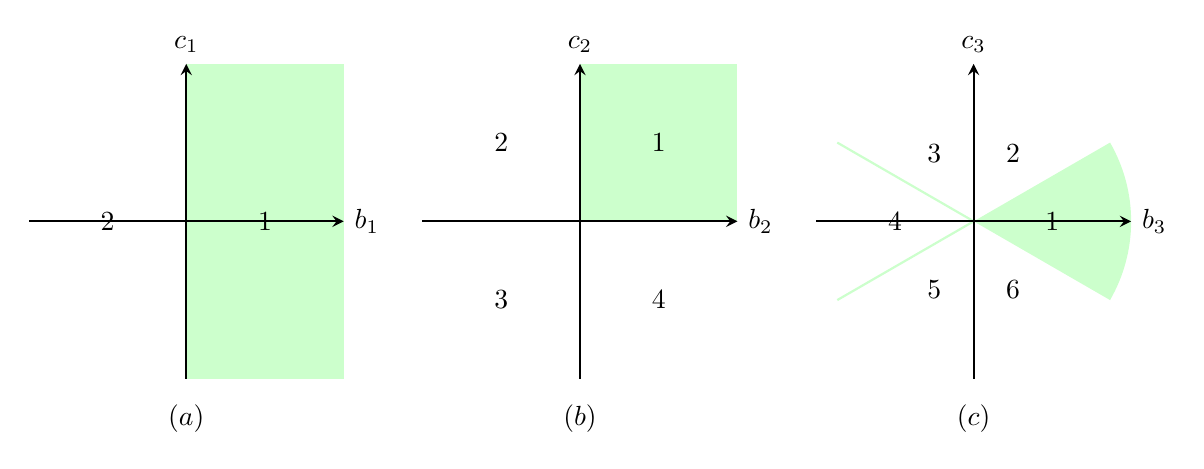
\begin{tikzpicture}

  % coordinates for the rectangle
  \coordinate (O1) at (0, 0);
  \coordinate (O2) at ($(O1) + (5, 0)$);
  \coordinate (O3) at ($(O2) + (5, 0)$);

  % draw the 1st configuration
  \node at ($(O1) + (0, -2.5)$) {$(a)$} ;
  \fill[fill=green!20] ($(O1) + (0, -2)$) rectangle ($(O1) + (2, 2)$);
  \node at ($(O1) + (1, 0)$) {1} ;
  \node at ($(O1) + (-1, 0)$) {2} ;

  \draw[color=black, thick] (O1) -- ($(O1) + (0, -2)$) ;
  \draw[->, >=stealth, color=black, thick] (O1) -- ($(O1) + (0, 2)$) node[above=0.2]{$c_1$};
  \draw[->, >=stealth, color=black, thick] (O1) -- ($(O1) + (2, 0)$) node[right=0.2]{$b_1$};
  \draw[color=black, thick] (O1) -- ($(O1) + (-2, 0)$);

  % draw the 2st configuration
  \node at ($(O2) + (0, -2.5)$) {$(b)$} ;
  \fill[fill=green!20] ($(O2) + (0, 0)$) rectangle ($(O2) + (2, 2)$);
  \node at ($(O2) + (1, 1)$) {1} ;
  \node at ($(O2) + (-1, 1)$) {2} ;
  \node at ($(O2) + (-1, -1)$) {3} ;
  \node at ($(O2) + (1, -1)$) {4} ;

  \draw[color=black, thick] (O2) -- ($(O2) + (0, -2)$) ;
  \draw[->, >=stealth, color=black, thick] (O2) -- ($(O2) + (0, 2)$) node[above=0.2]{$c_2$};
  \draw[->, >=stealth, color=black, thick] (O2) -- ($(O2) + (2, 0)$) node[right=0.2]{$b_2$};
  \draw[color=black, thick] (O2) -- ($(O2) + (-2, 0)$);


  % draw the 3rd configuration
  \node at ($(O3) + (0, -2.5)$) {$(c)$} ;
  \fill[fill=green!20] ($(O3) + (1.732, -1)$) arc (-30:30:2);
  \fill[fill=green!20] (O3) -- ($(O3) + (1.732, -1)$) -- ($(O3) + (1.732, 1)$) ;
  \node at ($(O3) + (1, 0)$) {1} ;
  \node at ($(O3) + (0.5, 0.866)$) {2} ;
  \node at ($(O3) + (-0.5, 0.866)$) {3} ;
  \node at ($(O3) + (-1, 0)$) {4} ;
  \node at ($(O3) + (-0.5, -0.866)$) {5} ;
  \node at ($(O3) + (0.5, -0.866)$) {6} ;

  \draw[color=green!20, thick](O3) -- ($(O3) + (-1.732, 1)$) ;
  \draw[color=green!20, thick](O3) -- ($(O3) + (-1.732, -1)$) ;

  \draw[color=black, thick] (O3) -- ($(O3) + (0, -2)$) ;
  \draw[->, >=stealth, color=black, thick] (O3) -- ($(O3) + (0, 2)$) node[above=0.2]{$c_3$};
  \draw[->, >=stealth, color=black, thick] (O3) -- ($(O3) + (2, 0)$) node[right=0.2]{$b_3$};
  \draw[color=black, thick] (O3) -- ($(O3) + (-2, 0)$);

\end{tikzpicture}
\endpgfgraphicnamed

\end{document}
